% This file was created by matlab2tikz.
%
%The latest updates can be retrieved from
%  http://www.mathworks.com/matlabcentral/fileexchange/22022-matlab2tikz-matlab2tikz
%where you can also make suggestions and rate matlab2tikz.
%

\documentclass[pt]{standalone}
\usepackage{amsmath}
\usepackage{graphicx}
\usepackage[pdf]{pstricks}
\usepackage{pgfplots}
\pgfplotsset{compat=newest}
\usepgfplotslibrary{fillbetween}
%% the following commands are needed for some matlab2tikz features
\usetikzlibrary{plotmarks}
\usetikzlibrary{arrows.meta}
\usepgfplotslibrary{patchplots}
\usetikzlibrary{decorations.text}
\usetikzlibrary{shapes.multipart}
%\usetikzlibrary{external}
%\tikzexternalize % activate!

\begin{document}
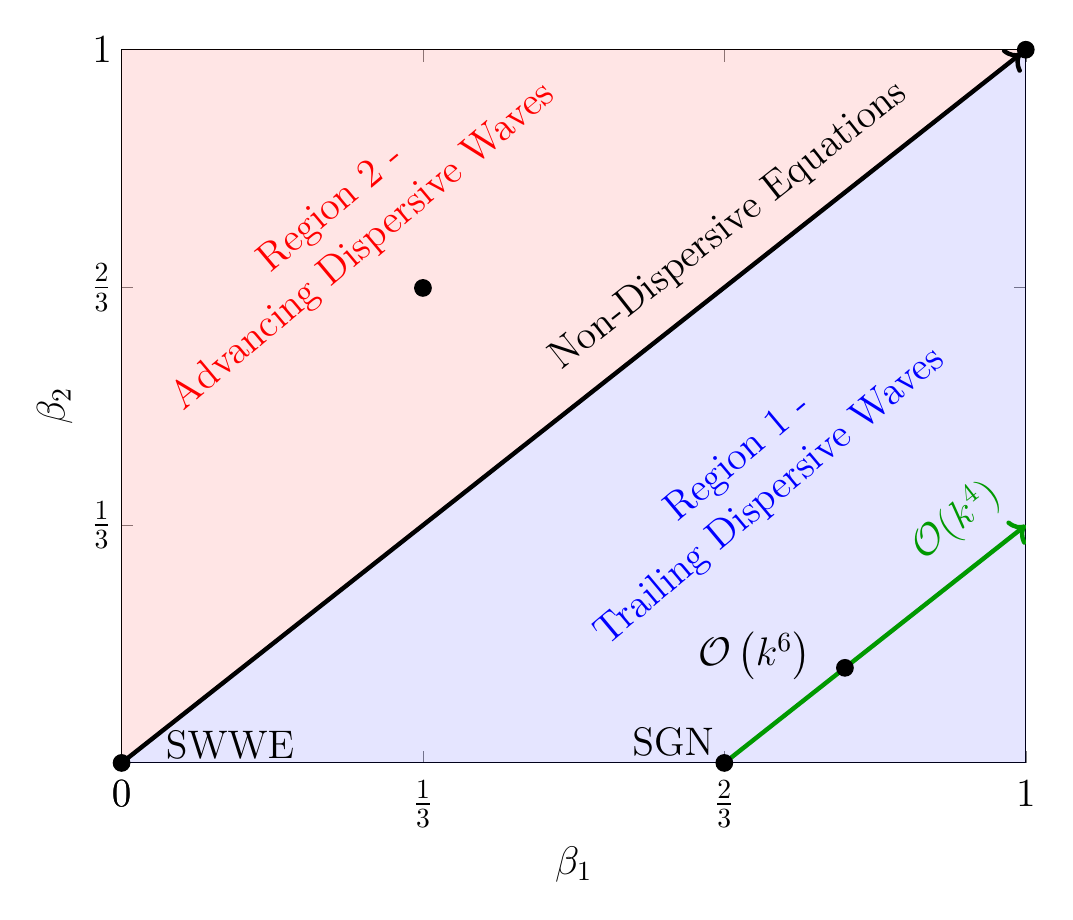
\begin{tikzpicture}[every text node part/.style={align=center}]
\tikzstyle{every node}=[font=\Large]
\begin{axis}[%
width=4.521in,
height=3.566in,
at={(0.758in,0.481in)},
scale only axis,
xmin=0,
xmax=1,
xtick={0,0.33333,0.66666,1},
xticklabels = {$0$,$\frac13$,$\frac23$,$1$},
xlabel={\Large $\beta_1$},
extra x ticks=0,
ymin=0,
ymax=1,
ytick={0.33333,0.66666,1},
yticklabels = {$\frac13$,$\frac23$,$1$},
ylabel={\Large $\beta_2$},
axis background/.style={fill=white},
xticklabel style = {yshift=-0.1cm}
];
\addplot+[name path=Above,mark=none, draw=none] coordinates {(0,1) (1,1)};


\draw[->,black,ultra thick] (0,0) --   (0.995,0.995) ;
\addplot[draw=none,blue,decoration={text along path,
	text={|\Large| Non-Dispersive Equations},
	raise=3ex,
	text color={black},
	text align={left indent={0.5\dimexpr\pgfdecoratedpathlength\relax}}},
postaction={decorate}]
coordinates {(0,0) (1,1)};

\path[name path=Critical ] (0,0) -- (1,1) ;

\draw[->,green!60!black,ultra thick] (0.6666666,0) --   (1,0.3333) ;

\addplot[draw=none,blue,decoration={text along path,
	text={|\Large| {$\mathcal{O}$}{$($}{$k^4)$} {} },
	raise=3ex,
	text color={green!60!black},
	text align={left indent={0.7\dimexpr\pgfdecoratedpathlength\relax}}},
postaction={decorate}]
coordinates {(0.6666666,0) (1,0.3333)};

\node[rotate = 40,blue] at (axis cs: 0.7,0.4) {Region 1 - \\ Trailing Dispersive Waves };
\node[rotate = 40,red] at (axis cs: 0.25,0.75) {Region 2 - \\ Advancing Dispersive Waves};


\addplot+[name path=Below,mark=none, draw=none] coordinates {(0,-0.1) (1,-0.1)};
\addplot[blue,opacity=0.1] fill between[of=Critical and Below];
\addplot[red,opacity=0.1] fill between[of=Critical and Above];


\addplot[only marks, mark size = 3pt] coordinates {(0,0) (0.6666,0) (0.79999,0.133333) (0.3333,0.666)(1,1)};
\node[] at (axis cs: 0.12,0.025) {SWWE};
\node[] at (axis cs: 0.61,0.03) {SGN};
\node[] at (axis cs: 0.7,0.15) {$\mathcal{O}\left(k^6\right)$};


\end{axis}

\end{tikzpicture}%

\end{document}